\documentclass[12pt]{article}
\usepackage{blindtext}
\usepackage[en,bordered]{uni-style}
\usepackage{uni-math}
\usepackage{subcaption}
\usepackage{array}

\title{Sentiment Analysis on Tweets of Stocks}
\prof{Dr. Khalaj}
\department{Department of Electrical Engineering}
\subtitle{Foundations of Data Science}
\subject{Project Report}
\info{
    \begin{tabular}{lr}
        Arad Mahdinejad Kashani & 400102028\\
    \end{tabular}
}
\date{\today}
\usepackage{uni-code}
\usepackage{graphicx}
\graphicspath{{pictures/}}
    
\begin{document}
\maketitlepage
\maketitlestart

\section{Introduction}
I did use Git for this project. I have messaged you on Telegram
so as to add you to my private repository. If needed, you can
contact my Telegram at \textit{@aradmnk}. Not much is happening, though.
There are only 4 python notebooks and the .csv file for the web-crawler
(`divar.csv', because I crawled `divar.ir').

The process is also documented in the notebook files themselves. 
There is text, and the code is segmented by the tasks in each 
phase of the project, so hopefully it is readable.
There are 4 notebook files, for the 3 phases and 1
for the bonus points.


\pagebreak

\section{Phase 1}
After reading the files, I made a realization that there exists a
certain tag (referred to a \textbf{CashTag \$} in the paper mentioned
in the project documentation) in the df[`text'] column. I used regex
to separate them in a different column and used that from then on.

\subsection{Task 1}

\begin{qsolve}[Task]
    Find the most and least tweeted stocks.
\end{qsolve}

\begin{figure}[h!]
    \centering
    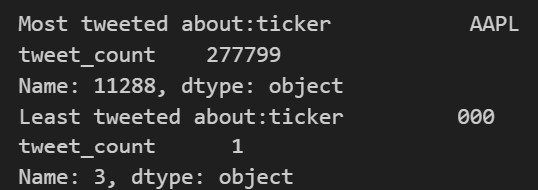
\includegraphics[width=.7\textwidth]{P1.1.jpg}
    \caption{Most and least stocks}
    \label{fig:1.1}
\end{figure}

As we can see, the most tweeted about stocks is \textbf{Apple Inc. \textit{(AAPL)}}.
The least tweeted about is irrelevant because there existed many tickers with
only 1 tweet (I checked it manually, it is not included in the notebook).

\begin{qsolve}[Task]
    Segment the companies based on tweet counts.
\end{qsolve}

\begin{figure}[h!]
    \centering
    \begin{subfigure}{.5\textwidth}
        \centering
        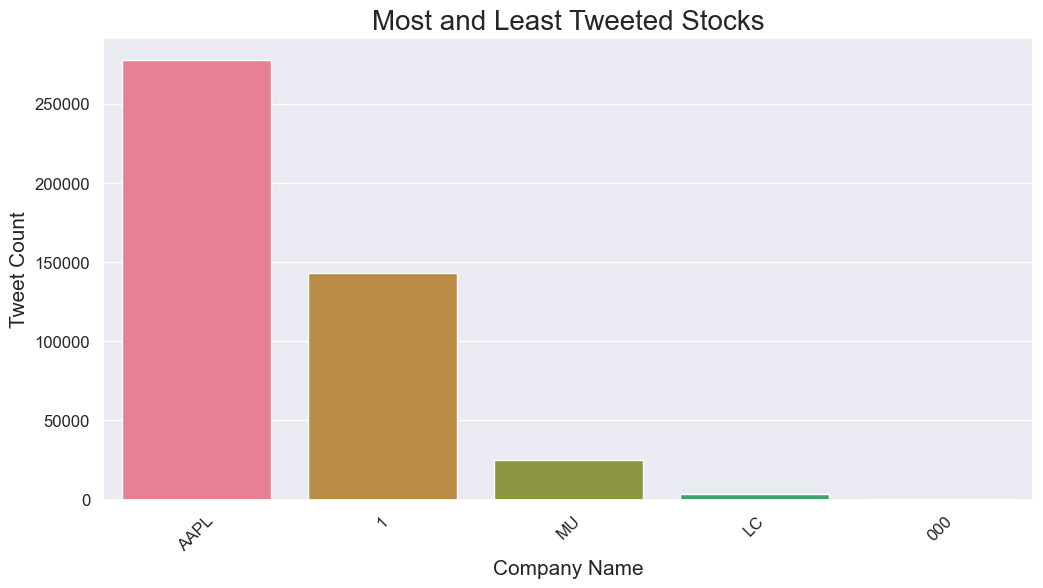
\includegraphics[width=.7\textwidth]{P1.1.2.png}
        \caption{Some companies and their respective tweet counts}
        \label{fig:1.1.2}
    \end{subfigure}%
    \begin{subfigure}{.5\textwidth}
        \centering
        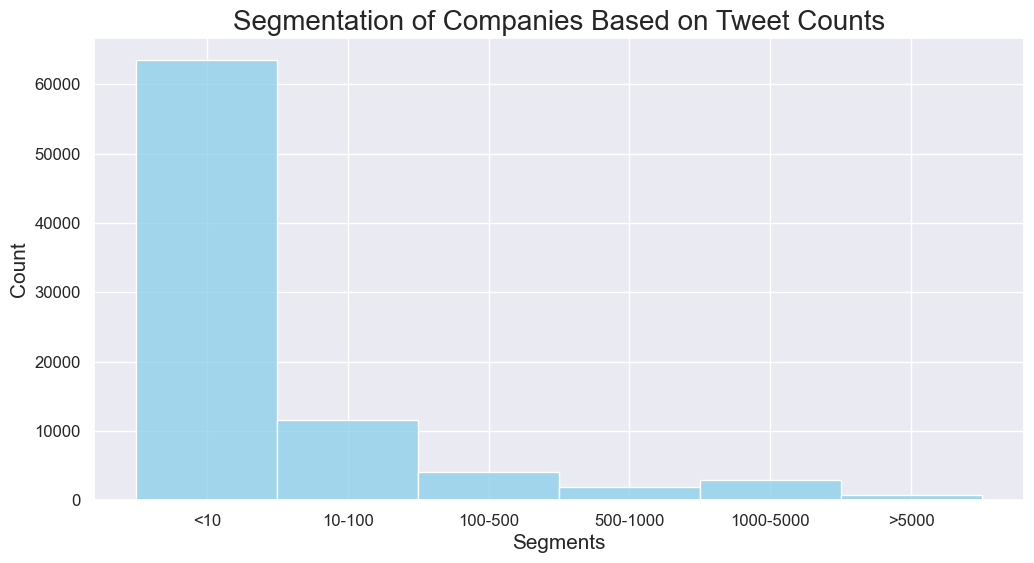
\includegraphics[width=.7\textwidth]{P1.1.3.png}
        \caption{Segmentation of the companies}
        \label{fig:1.1.3}
    \end{subfigure}
    \caption{}
\end{figure}

The middle companies of \textit{3.(a)} were 
hand picked from the middle, by index.

\pagebreak

\subsection{Task 2}

\begin{qsolve}[Task]
    Statistics on distributions of 5 individual 
    stocks over time. Choose the individual stocks to 
    perform reflect different sectors of the economy.
\end{qsolve}

\begin{figure}[h!]
    \centering
    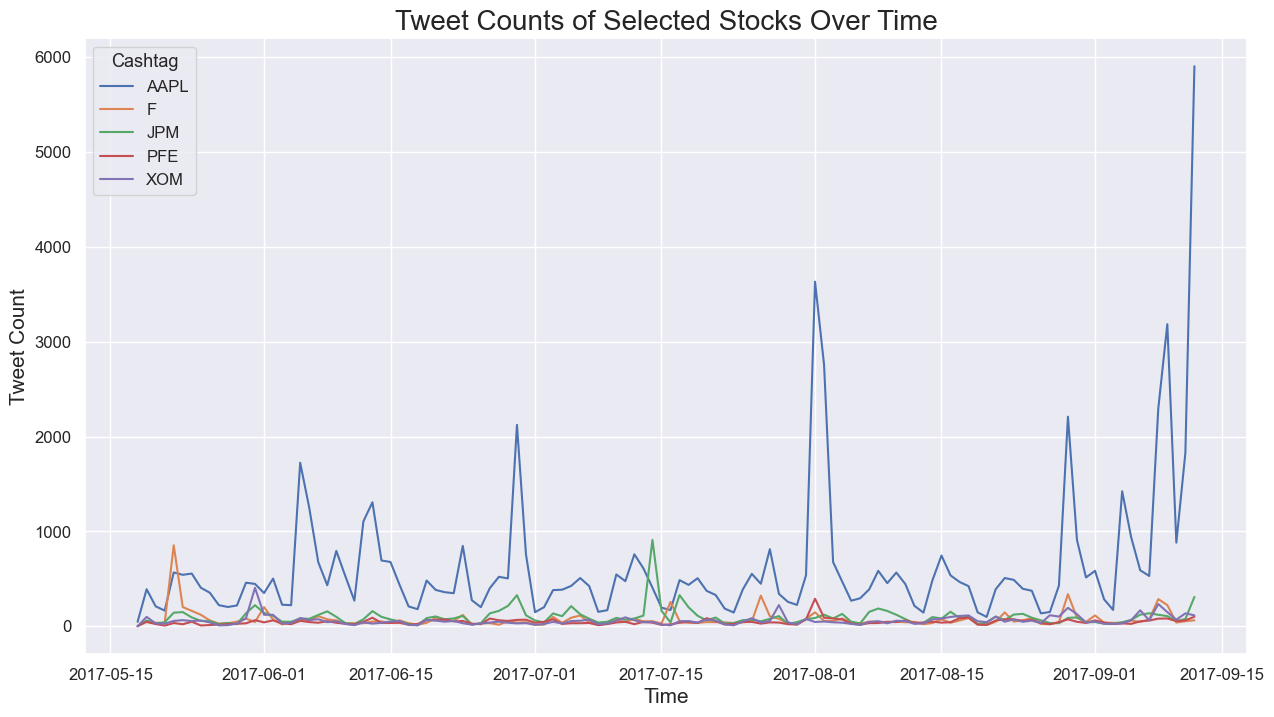
\includegraphics[width=1\textwidth]{P1.2.png}
    \caption{Individual stock distributions}
    \label{fig:1.2}
\end{figure}

I manually chose \textbf{Apple} (Technology), \textbf{ExxonMobil} (Energy), 
\textbf{Pfizer} (Healthcare), \textbf{JPMorgan Chase} (Financial), 
and \textbf{Ford} (Automotive).

\pagebreak

\subsection{Task 3}

\begin{qsolve}[Task]
    Statitistics on distributions of all financial tweets over time.
\end{qsolve}

\begin{figure}[h!]
    \centering
    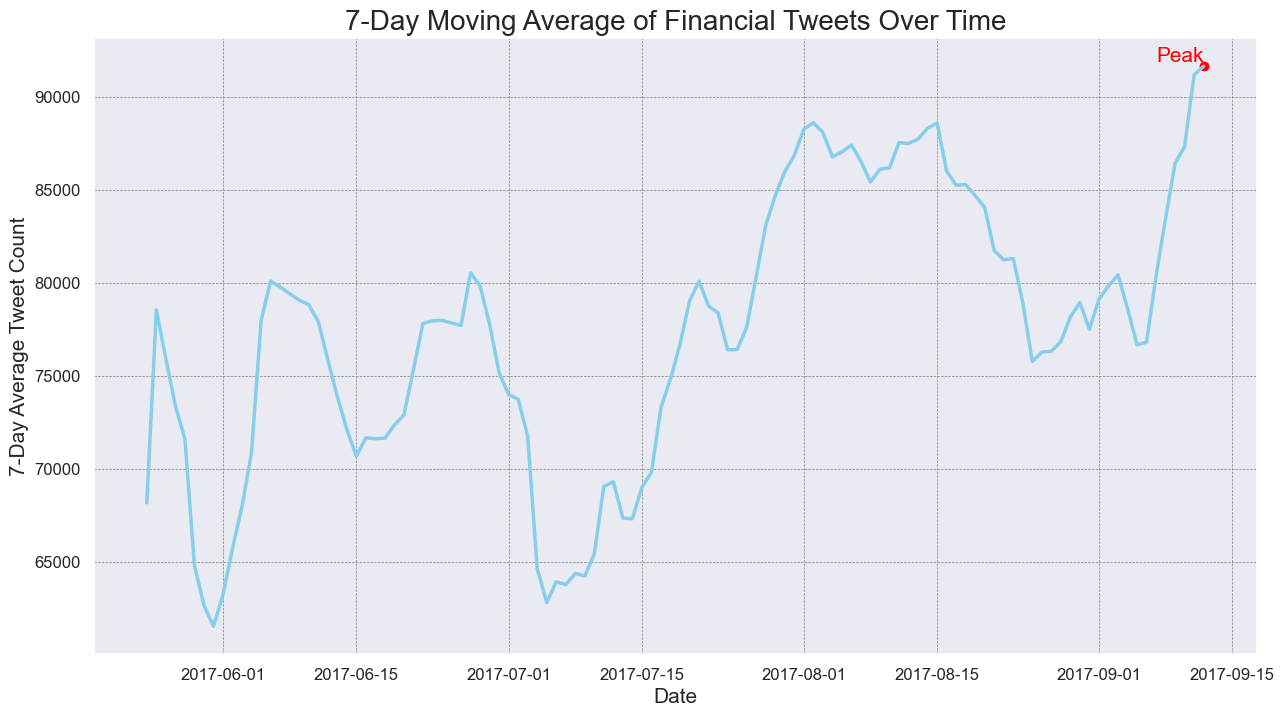
\includegraphics[width=1\textwidth]{P1.3.png}
    \caption{7-day average of all financial tweets over time}
    \label{fig:1.3}
\end{figure}

For this one I took on a 7-day moving average approach, just for
the sake of doing it.

\pagebreak

\subsection{Task 4}

\begin{qsolve}[Task]
    Statistics on distributions of retweets per tweets including 
    individual stocks (at least 2 chosen stocks) over time.
\end{qsolve}

\begin{figure}[h!]
    \centering
    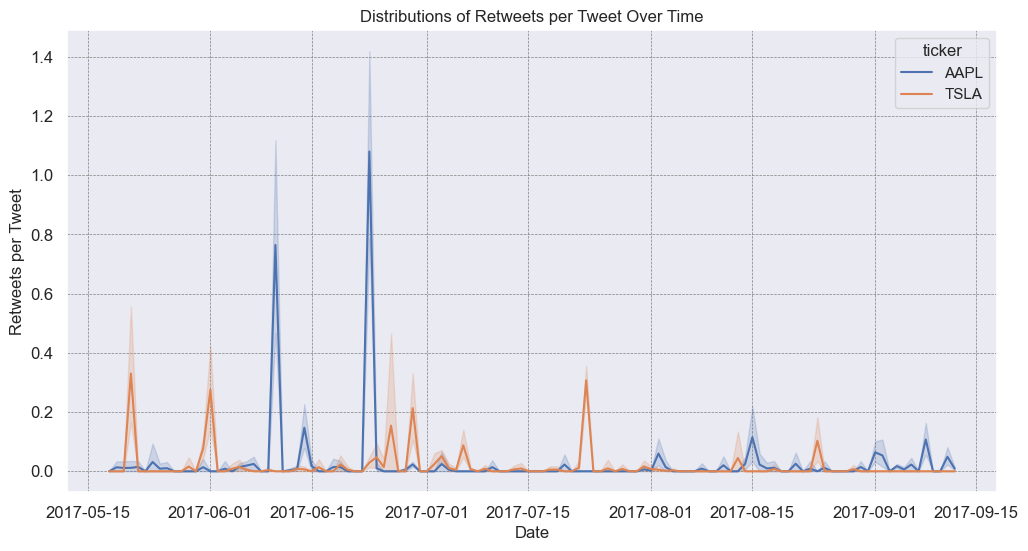
\includegraphics[width=1\textwidth]{P1.4.png}
    \caption{Distribution of retweets-per-tweet of \textbf{AAPL} and \textbf{TSLA} over time}
    \label{fig:1.4}
\end{figure}

I used Apple Inc. \textbf{(AAPL)} and Tesla Inc. \textbf{(TSLA)},
because I saw those in the demos and decided to use them for some reason.

\pagebreak

\subsection{Task 5}

\begin{qsolve}[Task]
    Statistics on most important financial information on 
    individual stocks (at least 2 chosen stocks) computed 
    solely from the financial information (not the tweets).
\end{qsolve}

\begin{figure}[h!]
    \centering
    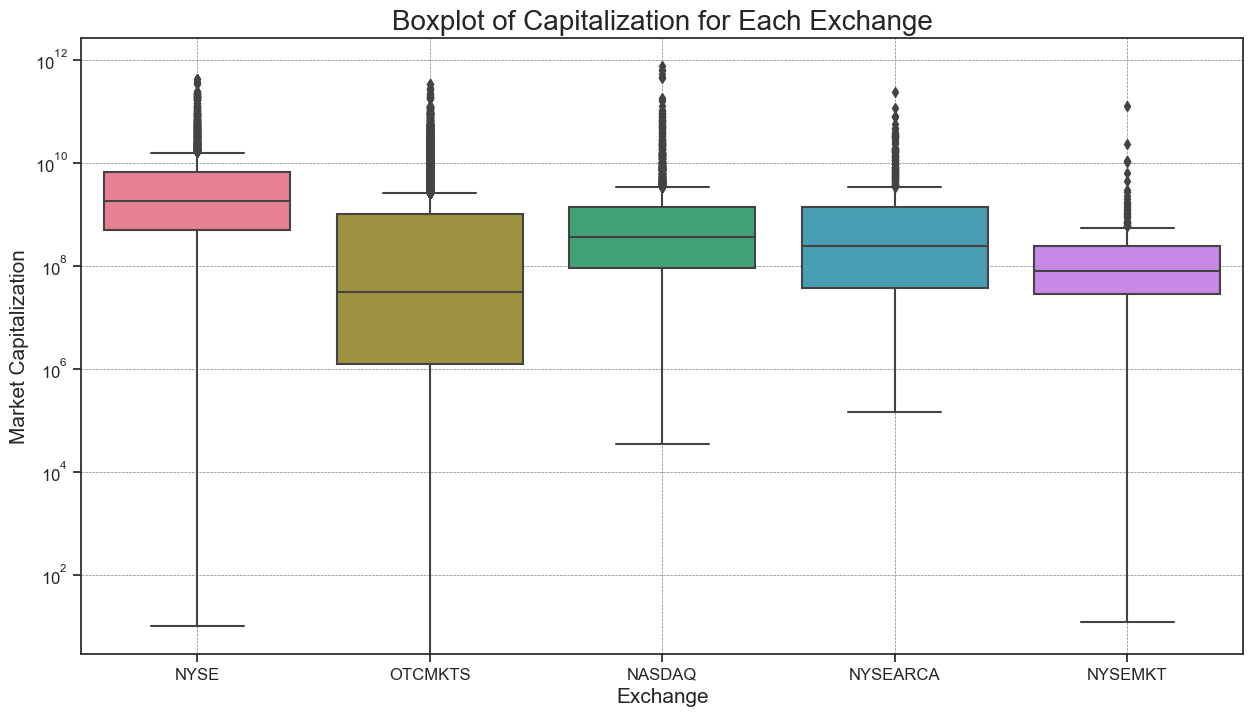
\includegraphics[width=1\textwidth]{P1.5.png}
    \caption{Box-plot of capitalizations per exchange (logarithmic)}
    \label{fig:1.5}
\end{figure}

The data for the box-plots was obtained from the 
`companies.csv' file.

\begin{figure}[h!]
    \centering
    \begin{subfigure}{.4\textwidth}
        \centering
        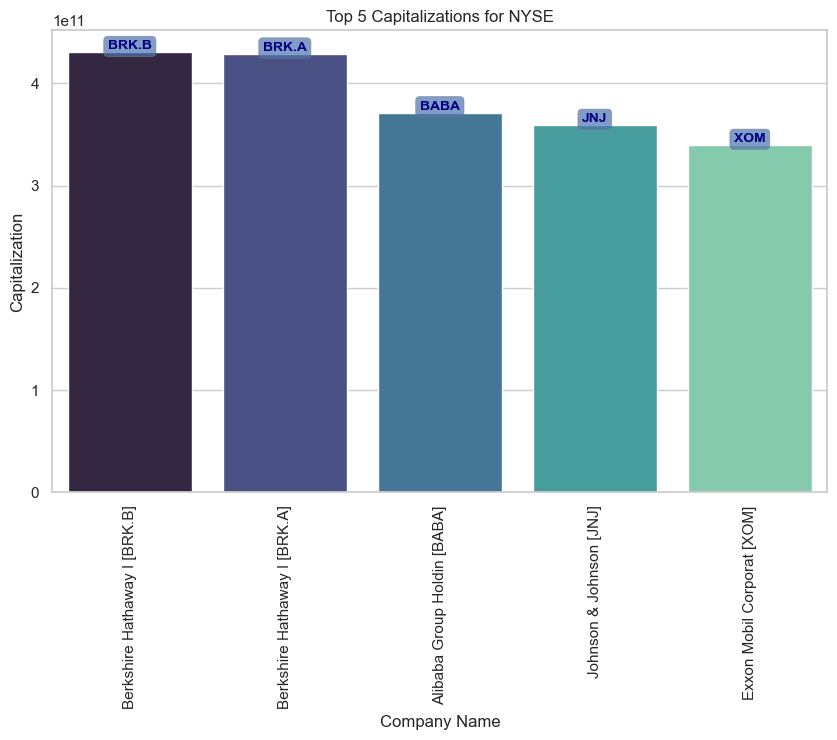
\includegraphics[width=.7\textwidth]{P1.5.1.png}
        \caption{NYSE}
        \label{fig:1.5.1}
    \end{subfigure}%
    \begin{subfigure}{.4\textwidth}
        \centering
        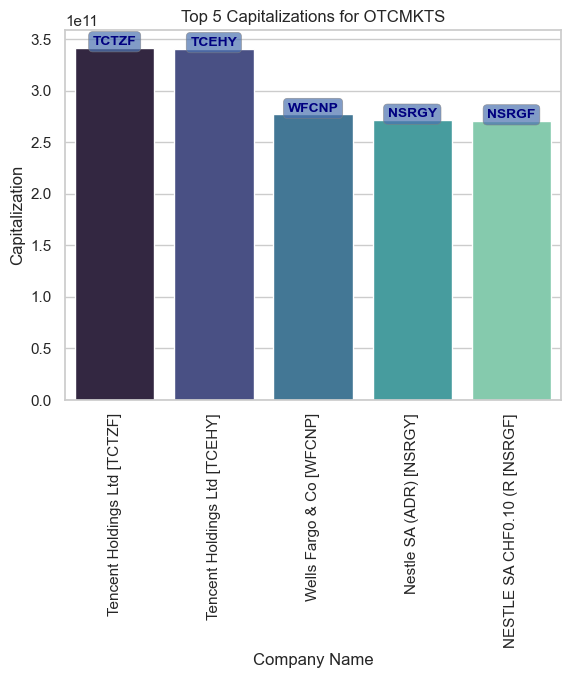
\includegraphics[width=.7\textwidth]{P1.5.2.png}
        \caption{OTCMKTS}
        \label{fig:1.5.2}
    \end{subfigure}

    \begin{subfigure}{.4\textwidth}
        \centering
        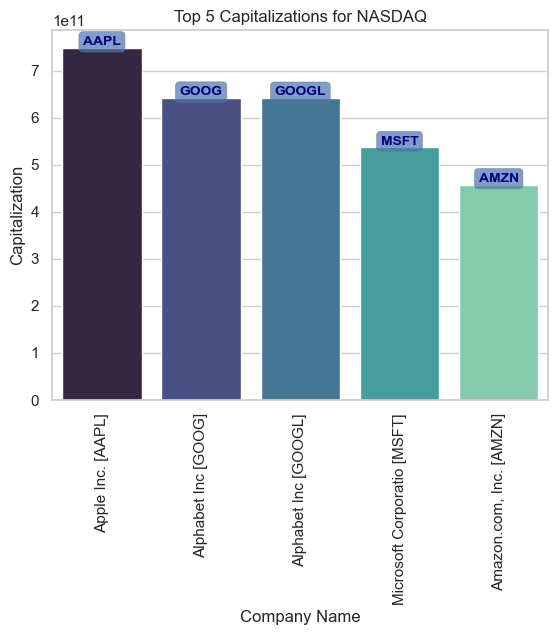
\includegraphics[width=.7\textwidth]{P1.5.3.png}
        \caption{NASDAQ}
        \label{fig:1.5.3}
    \end{subfigure}%
    \begin{subfigure}{.4\textwidth}
        \centering
        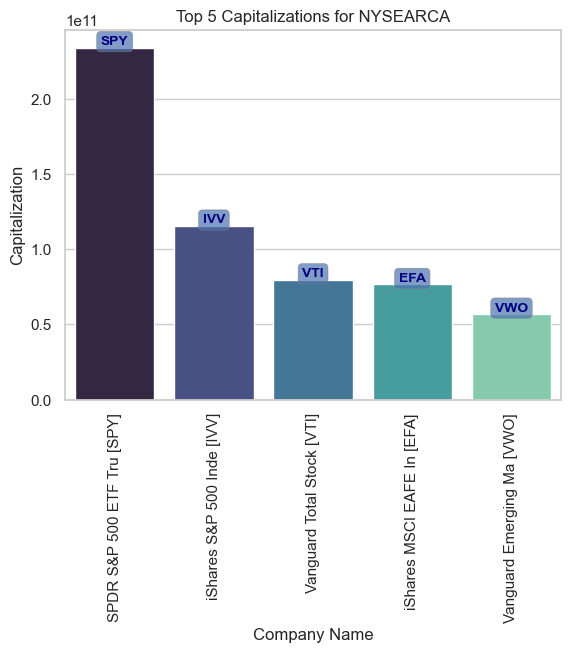
\includegraphics[width=.7\textwidth]{P1.5.4.png}
        \caption{NYSEARCA}
        \label{fig:1.5.4}
    \end{subfigure}
    \begin{subfigure}{.7\textwidth}
        \centering
        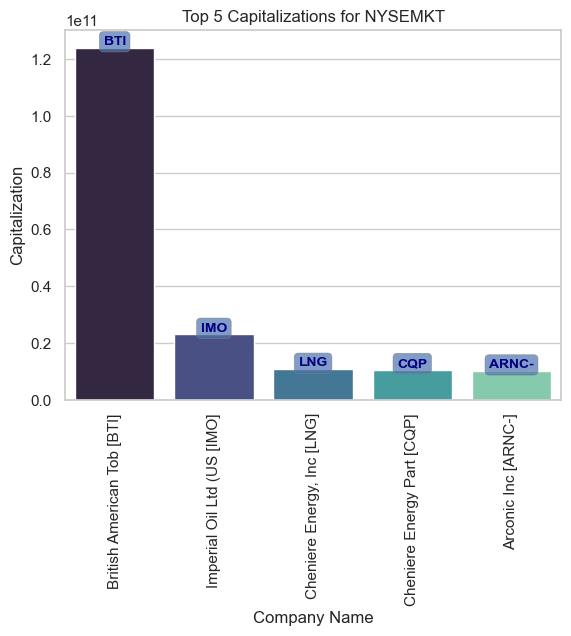
\includegraphics[width=.7\textwidth]{P1.5.5.png}
        \caption{NYSEMKT}
        \label{fig:1.5.5}
    \end{subfigure}
    \caption{Top 5 capitalizations for each exchange}
\end{figure}

\pagebreak

\subsection{Task 6}

\begin{qsolve}[Task]
    Time series movement directions through time for individual 
    stocks (at least 2). Choose companies you are familiar with. 
    Try to explain the reason behind these directions from real 
    world news.
\end{qsolve}

\begin{figure}[h!]
    \centering
    \begin{subfigure}{.4\textwidth}
        \centering
        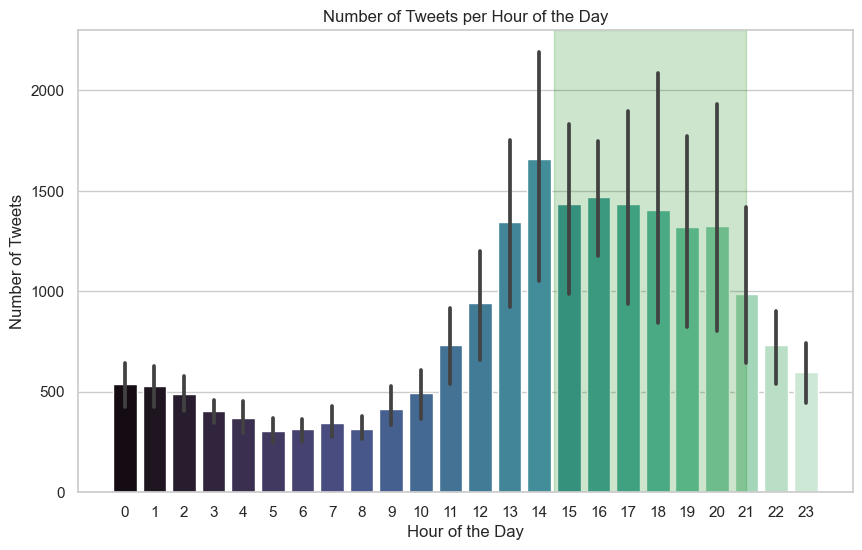
\includegraphics[width=.7\textwidth]{P1.6.3.png}
        \caption{Number of tweet per hour of the day}
        \label{fig:1.6.3}
    \end{subfigure}%
    \begin{subfigure}{.4\textwidth}
        \centering
        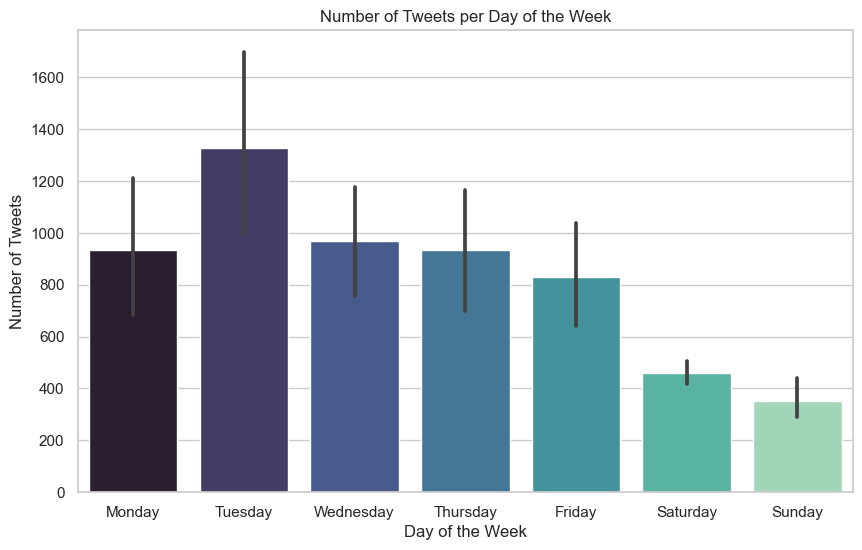
\includegraphics[width=.7\textwidth]{P1.6.2.png}
        \caption{Number of tweet per day of the week}
        \label{fig:1.6.2}
    \end{subfigure}
    \begin{subfigure}{.7\textwidth}
        \centering
        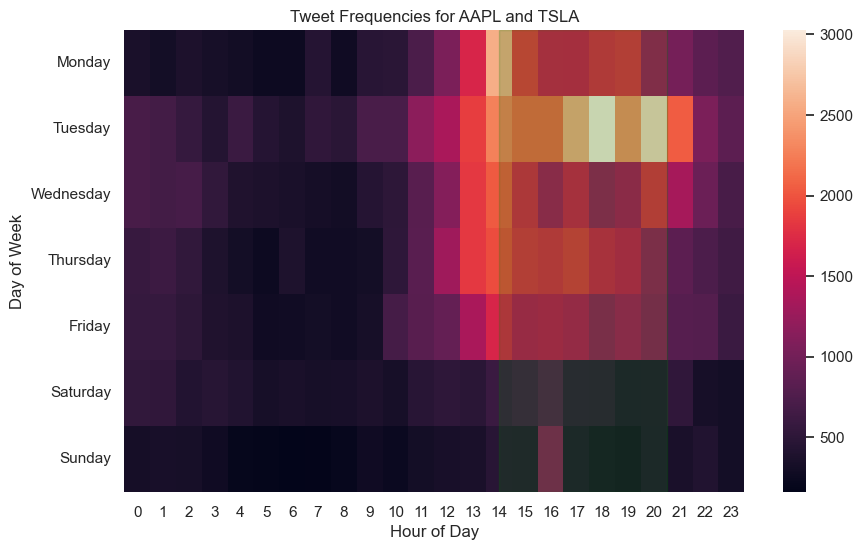
\includegraphics[width=.7\textwidth]{P1.6.1.png}
        \caption{Tweet frequencies per day of the week and hour of the day}
        \label{fig:1.6.1}
    \end{subfigure}
    \caption{Time series movement for number of tweets}
\end{figure}

\begin{itemize}
    \item In figure \textit{8.(a)}, we can see a peak at the trading hours 
    (highlighted green) and even an hour before trading hours. A psychological
    analysis may be that the traders will be checking tweeter an hour before trading
    to see how to market may be going, or maybe those interested in selling their shares
    may try to persuade buyers to buy their share of stock.

    \item In figure \textit{8.(b)}, we can see a drop on the days off (Saturday and Sunday).
    Tuesday seems to have a peak as well, but I lack knowledge of the
    market to be able to analyize why!

    \item In figure \textit{8.(c)}, we can see the joint distribution per day and week.
    The most frequent trading time is the trading hours in the working days.
    Tuesdays seem to be very heated (and I do not know why)!
\end{itemize}

\pagebreak

\subsection{Task 7}

\begin{qsolve}[Task]
    Co-occurence of various stocks in the same tweets.
\end{qsolve}

\begin{figure}[h!]
    \centering
    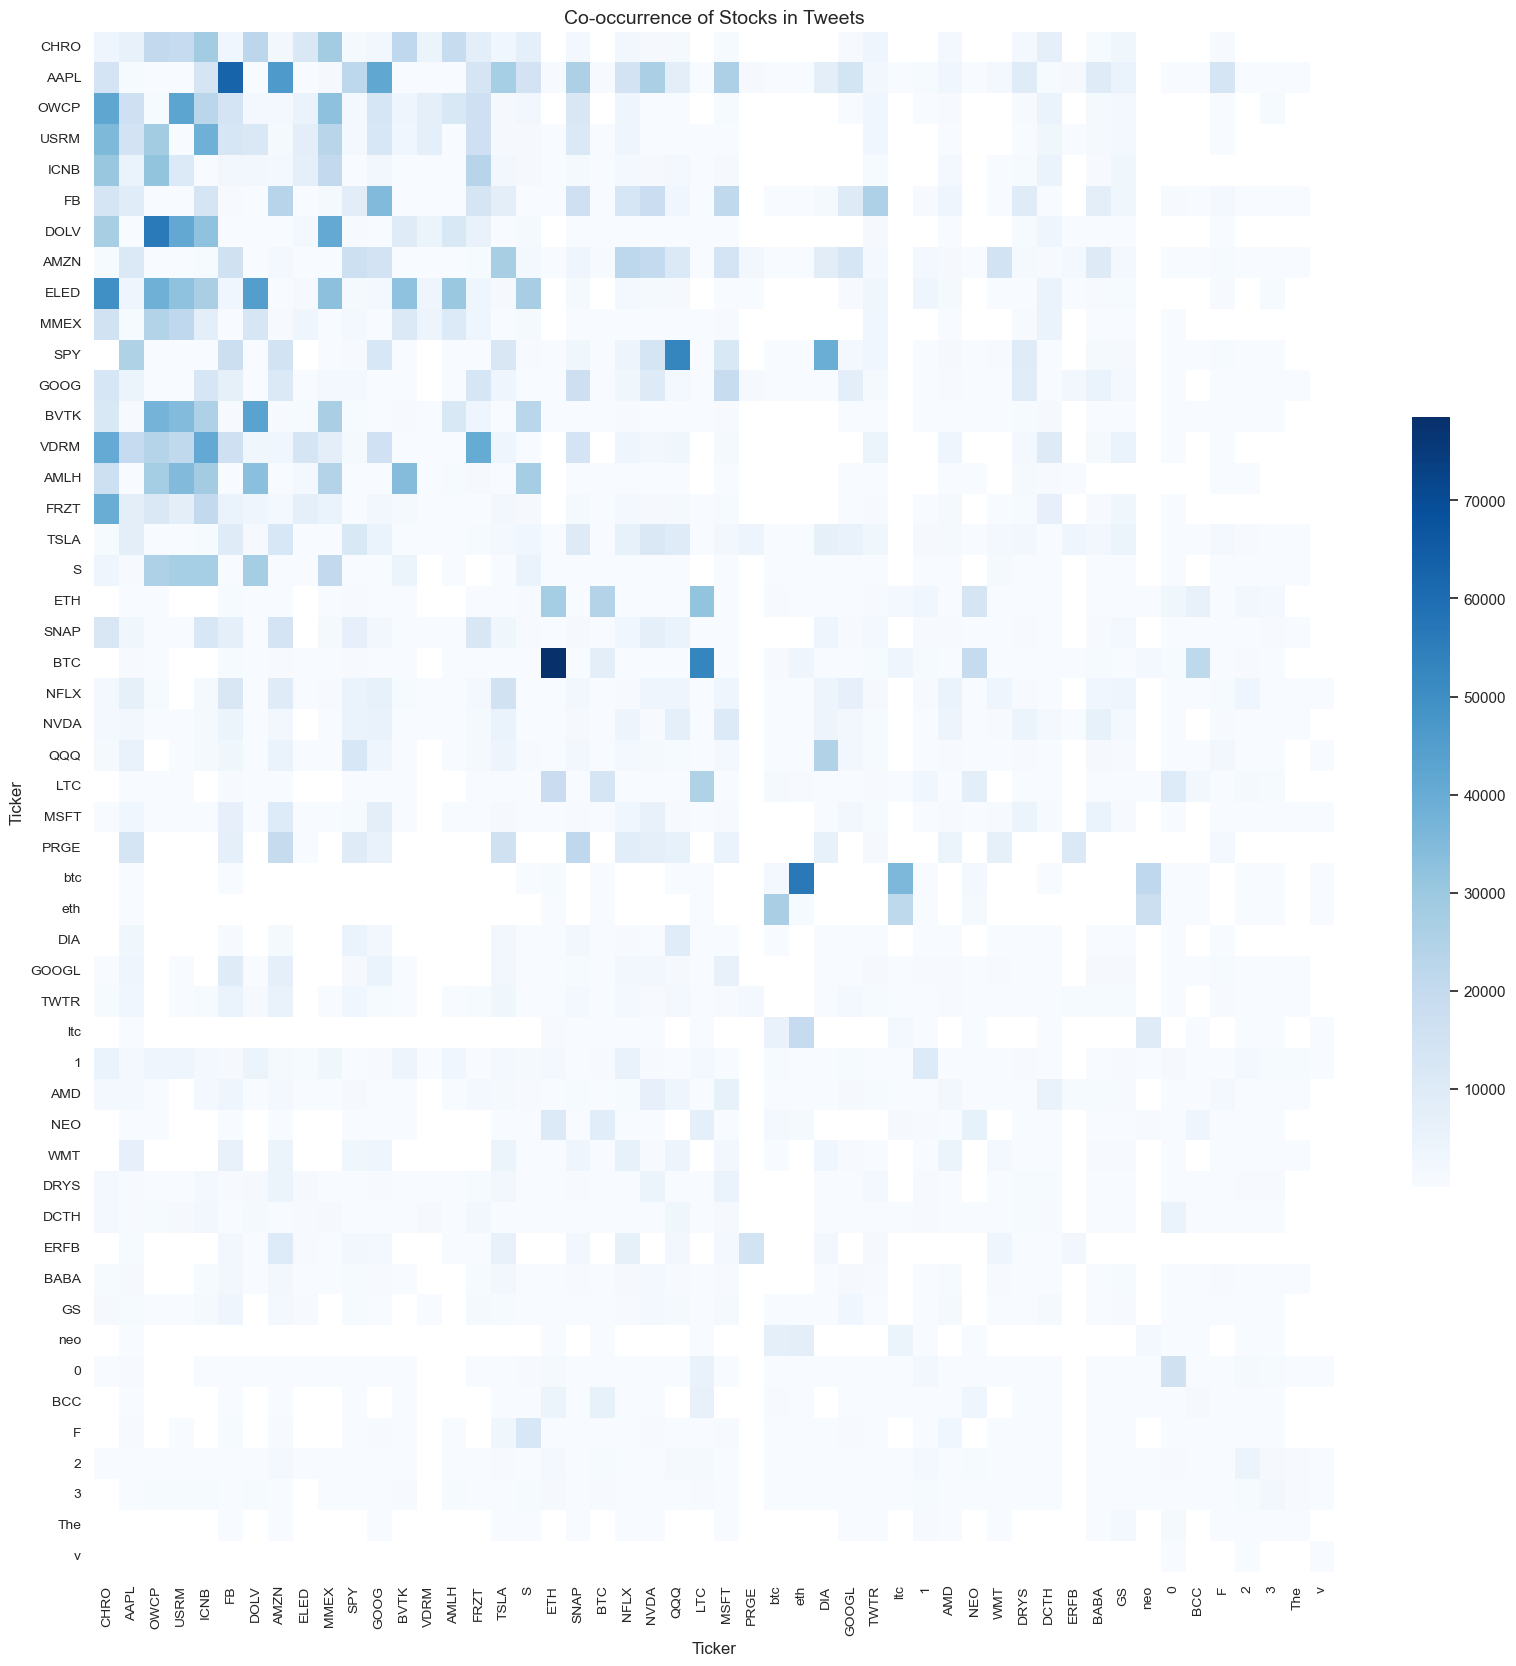
\includegraphics[width=1\textwidth]{P1.7.png}
    \caption{Co-occurence matrix of various stocks in the same tweet}
    \label{fig:1.7}
\end{figure}

The process is very time-consuming. I had to get the top 50 most 
common tickers to be able to computationally handle the task. It seems
\textbf{ETH} and \textbf{BTC} occur the most together. Another contestant
to that is \textbf{AAPL} and \textbf{FB}.

\section{Phase 2}
After reading the data and processing the time-series data, I was ready
to begin the training process. The problem was that the data size was
too huge for me to work with properly (as I tend to do the work with
trial and error), so I sampled the data and worked with a $N=100,000$
sample dataframe. All of the models were trained and evaluated this way.

I also had to use \textbf{Kaggle} for this Phase (and the next), because
my device did not have a usable GPU for training the models; I only had
a GPU there. Hopefully the file directories will make more sense when
you read the notebook now.

\subsection{Cleaning the data}

\begin{qsolve}[Task]
    Clean the data.
    \begin{itemize}
        \item Removing duplicate values and useless data (both columns and rows).
        \item Handling upper/lower case, etc.
    \end{itemize}
\end{qsolve}

First the links were removed. Then, the hashtags were separated 
from the text data, and punctuation was removed from the tweet.
All non-english characters were removed, and tokenized with the
stop-words removed. The stop-words were obtained from nltk.stop\_words.

\pagebreak

\subsection{Bag Of Words}

\subsubsection{Support Vector Machine (SVM)}

\begin{tabular}{lr}
    Train accuracy & 86.71\%\\
    Validation accuracy & 52.25\%\\
    Test accuracy & 51.77\%\\
\end{tabular}

\begin{figure}[h!]
    \centering
    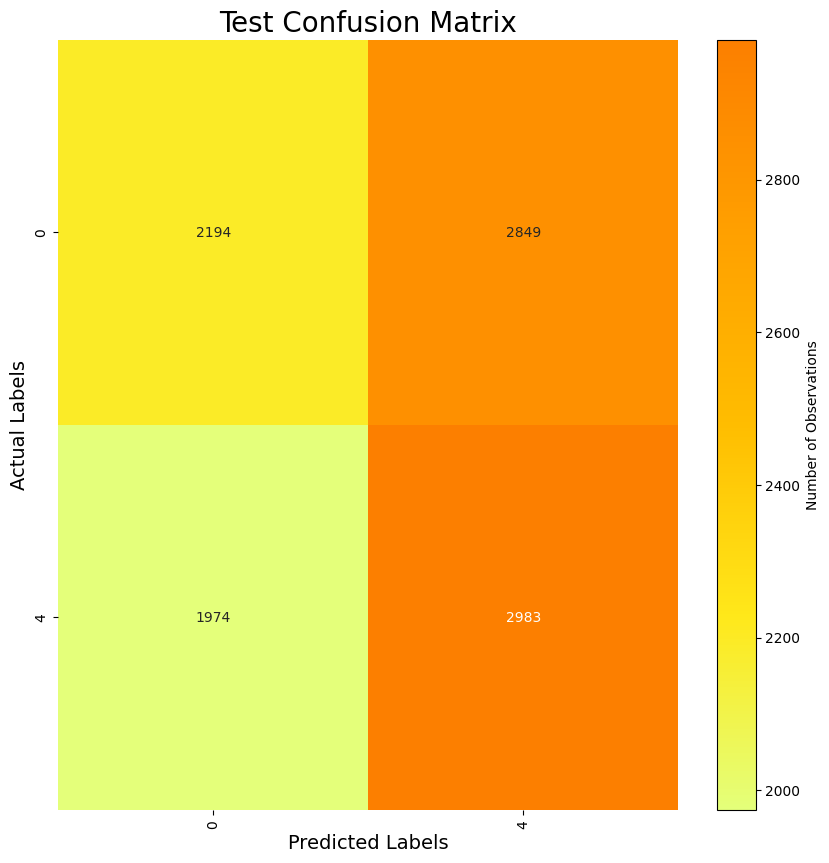
\includegraphics[width=.3\textwidth]{P2.BOW.1.png}
    \caption{SVM + BOW Confusion Matrix}
    \label{fig:2.BOW.1}
\end{figure}

\subsubsection{Random Forest}

\begin{tabular}{lr}
    Train accuracy & 96.43\%\\
    Validation accuracy & 52.12\%\\
    Test accuracy & 52.32\%\\
\end{tabular}

\begin{figure}[h!]
    \centering
    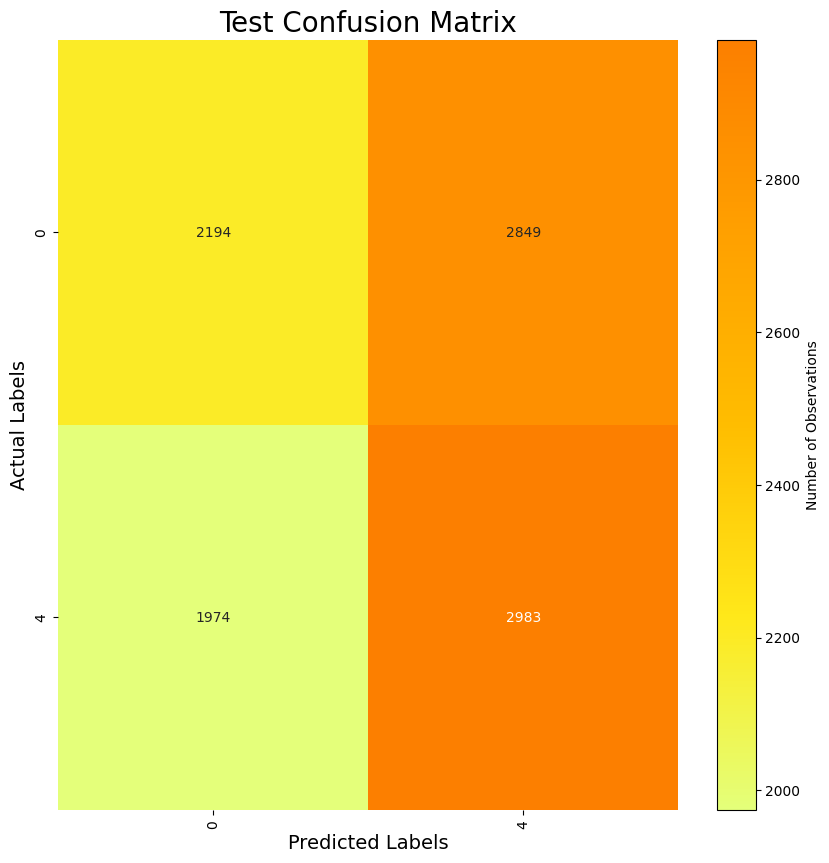
\includegraphics[width=.3\textwidth]{P2.BOW.1.png}
    \caption{Random Forest + BOW Confusion Matrix}
    \label{fig:2.BOW.2}
\end{figure}

The Random Forest already looks more promising, judging by the confusion matrices.
The main diagonal of the confusion matrix seems brighter. It seems
sentiment analysis is not linearly separable (what a surprise).

\pagebreak

\subsection{TF-IDF}

\subsubsection{Support Vector Machine (SVM)}

\begin{tabular}{lr}
    Train accuracy & 94.92\%\\
    Validation accuracy & 77.62\%\\
    Test accuracy & 77.27\%\\
\end{tabular}

\begin{figure}[h!]
    \centering
    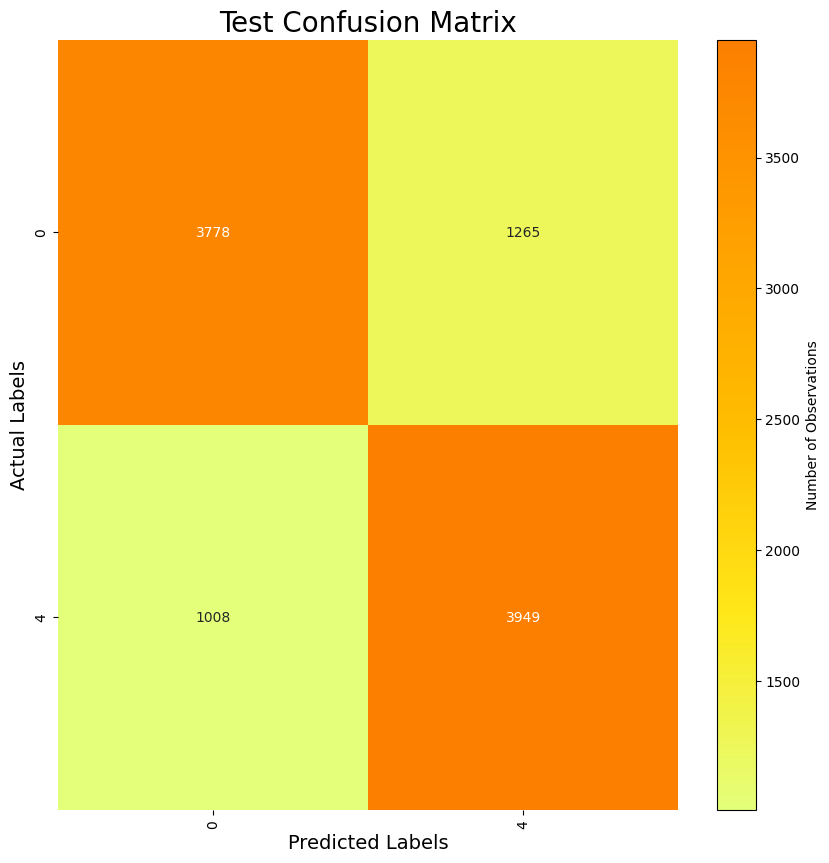
\includegraphics[width=.3\textwidth]{P2.TFIDF.1.png}
    \caption{SVM + TF-IDF Confusion Matrix}
    \label{fig:2.TDIDF.1}
\end{figure}

\subsubsection{Random Forest}

\begin{tabular}{lr}
    Train accuracy & 99.46\%\\
    Validation accuracy & 75.63\%\\
    Test accuracy & 75.54\%\\
\end{tabular}

\begin{figure}[h!]
    \centering
    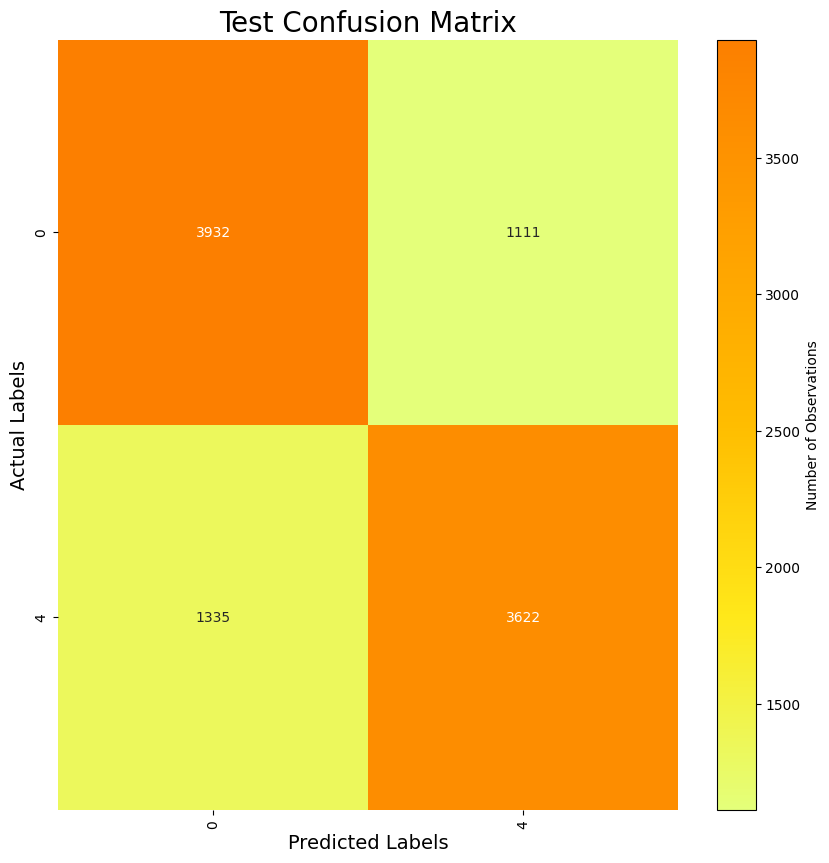
\includegraphics[width=.3\textwidth]{P2.TFIDF.2.png}
    \caption{Random Forest + TF-IDF Confusion Matrix}
    \label{fig:2.TFIDF.2}
\end{figure}

The Random Forest already looks more promising, judging by the confusion matrices, 
as the main diagonal of the confusion matrix seems brighter. TF-IDF
is already performing better than the BOW method.

\pagebreak

\subsection{SpaCy}
There is not much to say here really, except that I used the `textcat'
pipeline, already pre-prepared for our purpose (binary text-classification).

\begin{figure}[h!]
    \centering
    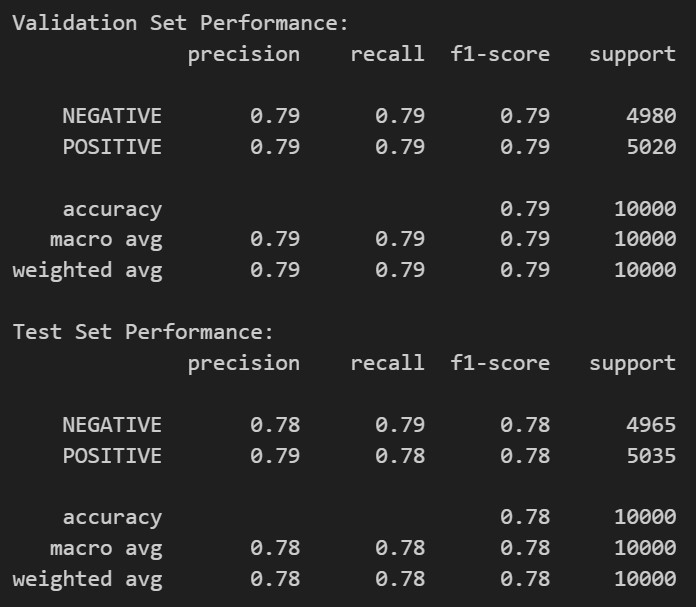
\includegraphics[width=.6\textwidth]{P2.SpaCy.jpg}
    \caption{SpaCy classifier metrics}
    \label{fig:P2.SpaCy}
\end{figure}

\pagebreak

\subsection{Fine-tuning HuggingFace: Distil-BERT}

For the next section, I chose not to use the GPT API (because I did not
have enough time to calculate the token and chose to accept risk)
and instead used a fine-tuned version of the Distil-BERT model from 
HuggingFace. The reason I used SpaCy, was the fact that I did not like
having two BERT models for this project.

\begin{tabular}{lr}
    Train accuracy & 99.06\%\\
    Validation accuracy & 78.95\%\\
    Test accuracy & 77.85\%\\
\end{tabular}

\begin{figure}[h!]
    \centering
    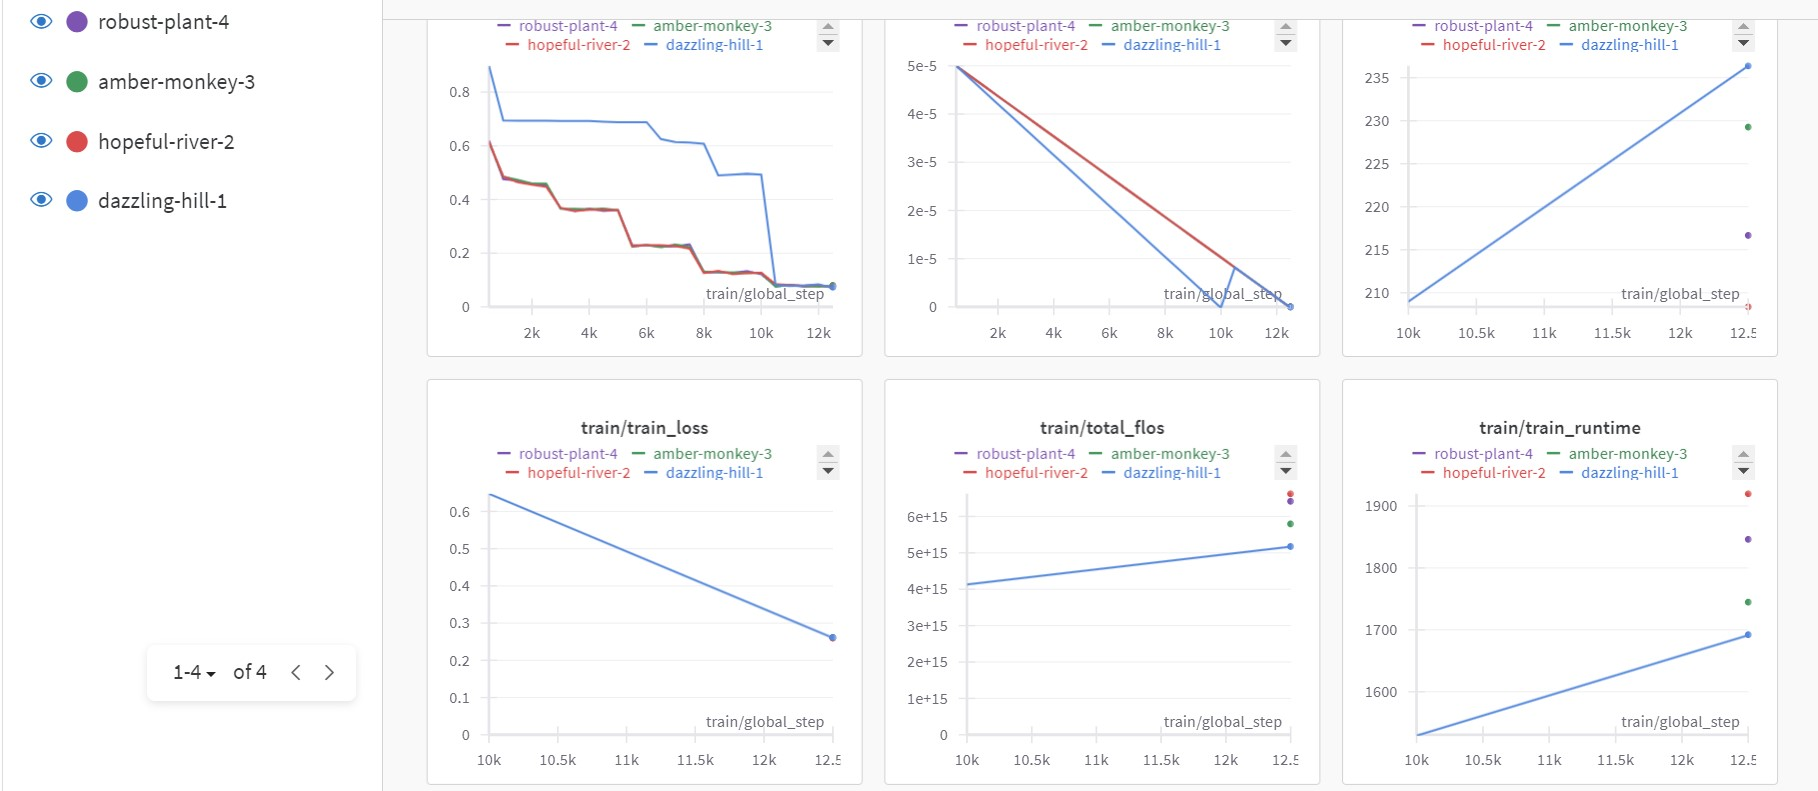
\includegraphics[width=1\textwidth]{P2.Distil-BERT.jpg}
    \caption{HuggingFace workspace dashboard (robust-plant-4 is the final model, purple)}
    \label{fig:P2.DistilBERT}
\end{figure}

\subsection{Comparison of Models}

Accuracy-wise, it can be easily shown that the last two models are better.
That was not too far-fetched, as BOW is weak and RF and SVM and other
traditional methods are not very practical in replicating the attention
mechanisms required for NLP and Sentiment Analysis. They \textit{can} work,
but deep methods with attention mechanisms (or other adjacency methods)
are better at doing this special task; as the task is not neccessarily simple.

The SpaCy model and the Distil-BERT model were saved and used for the next phase,
as they yielded the best results.

\pagebreak

\section{Phase 3}

\subsection{Applying Classifiers}

The main database is \textbf{very large}. I had to sample it again
to achieve my results in reasonable time. I again used $N=100,000$
samples, applied the CashTag(\$) extraction and used both of the
models on the preprocessed tweet texts.

\subsection{Pearson and Spearman Correlation}

\begin{qsolve}[Task]
    Using different correlation measures (at least 2 and you can use 
    libraries), find the correlation between the sentiments of each CashTag 
    and its value (from the financial data in the companies dataset) in a 
    time interval.
\end{qsolve}

As the task required a `time interval', I used the middle month
as a time to calculate the correlation. I used the `scipy.stats' 
library for these correlations.

\begin{figure}[h!]
    \centering
    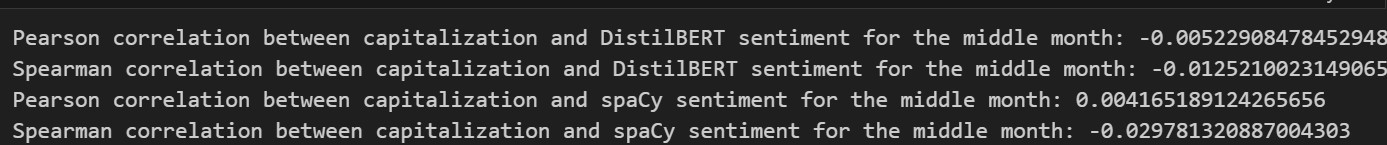
\includegraphics[width=1\textwidth]{P3.correlation.jpg}
    \caption{Spearman and Pearson correlations for 
    each model between sentiments and capitalizations}
    \label{fig:P3.correlation}
\end{figure}

\begin{qsolve}[Task]
    Using different correlation measures, find the correlation between 
    change of sentiments of CashTag and the number of tweets related to 
    that CashTag in the time series (By time series of tweets, we mean the 
    number of tweets per given time that was calculated in the first part).
\end{qsolve}

\begin{figure}[h!]
    \centering
    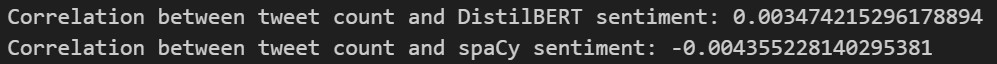
\includegraphics[width=1\textwidth]{P3.correlation.2.jpg}
    \caption{Correlation for 
    each model between sentiments and retweets-per-tweet}
    \label{fig:P3.correlation.2}
\end{figure}

I may or may not have forgotten to use two correlation measures\dots

The correlation amounts are very small, in general. Some of them are
negative as well. This \textit{may} have a meaning, but the correlations
I have arrived at are not meaningful/significant enough for conclusions.

\pagebreak

\subsection{Classifier Conflicts}

\begin{qsolve}[Task]
    Find examples where the classifiers do not agree on the sentiment of 
    the tweet and analyze the results and discuss where does each 
    classifier make mistakes.
\end{qsolve}

\begin{table}[h!]
    \centering
    \begin{tabular}{ || m{25em} | m{8em}| m{5em} || }
        \hline
        \textbf{Text} & \textbf{Distil-BERT} & \textbf{SpaCy} \\ 
        \hline

        At Home Group Inc \$HOME Forecasted to Earn Q4 2018 Earnings 
        of \$0.30 Per Share https://t.co/VDycVabjjq & NEGATIVE & POSITIVE\\
        \hline

        \$OCRX Company has begun dosing of the first patients in Part Two of 
        a Phase1/Phase 2a clinical trial of oral OCR-0… 
        https://t.co/csMCRZ2oBq & NEGATIVE & POSITIVE\\
        \hline

        SG Americas Securities LLC Cuts Position in Vector Group Ltd. \$VGR 
        https://t.co/7Rp2CfVfOo & NEGATIVE & POSITIVE\\
        \hline

        Dimensional Fund Advisors LP Has \$15.57 Million Position in Capital 
        City Bank Group \$CCBG https://t.co/x5hl85YeKQ & POSITIVE & NEGATIVE \\
        \hline

        Startin the week off with a bang. \$RGNX https://t.co/AX5RTRcGNh 
        TV\_TradingIdeas & POSITIVE & NEGATIVE \\
        \hline
    \end{tabular}
    \caption{Classifier disagreement examples}
    \label{table:P3.t1}
\end{table}

For the first, second, and the fourth examples, I personally cannot decide
on the sentiment as a human. However, for the third and fifth examples, I
think the SpaCy model is slightly weaker than the Distil-BERT model.
For instance in the fifth example, I think the model thinks that ``bang''
is a bad word because of guns and weapons; while the phrase ``starting off with a bang''
is a totally positive sentiment. Distil-BERT has managed to capture that.

\pagebreak

\subsection{Discussion}
\begin{qsolve}
    Discuss transfer learning and fine-tuning and how they can be used to 
    improve the overall effect of the project. Use your limited results 
    from the first part.
\end{qsolve}

\textbf{Transfer Learning} and \textbf{Fine-Tuning} are powerful techniques 
in machine learning that can significantly improve the performance of a 
model, especially when dealing with tasks where the available data is 
limited.

\textbf{Transfer Learning} is a technique where a pre-trained model, which 
has been trained on a large-scale dataset, is used as a starting point for 
a related task. The idea is to leverage the knowledge that the model has 
already learned from the large dataset to perform the new task. This is 
particularly useful when the new task has limited data, as it allows the 
model to generalize better.

For example, in the context of this project, a pre-trained language model 
like BERT or Distil-BERT, which has been trained on a large corpus of text, 
can be used as a starting point for sentiment analysis. The pre-trained 
model already understands the semantics of the language to a great extent, 
which can be leveraged to understand the sentiment of the tweets.

\textbf{Fine-Tuning} is a process that adjusts the pre-trained model to the new 
task. After initializing our model with the pre-trained weights, we 
continue training the model on our specific task (like sentiment analysis 
in this project). During this process, the model learns to adjust its
weights and biases to specialize on the new task.

In the context of this project, fine-tuning can be used to adapt the 
pre-trained language model to the specific language and style used in the 
tweets. This can lead to a more accurate sentiment prediction.

In summary, transfer learning and fine-tuning can greatly improve the 
performance of the model in this project by leveraging the knowledge from 
large-scale pre-training and adapting it to the specific task of tweet 
sentiment analysis. This can lead to more accurate sentiment predictions, 
which in turn can improve the correlation analysis between tweet 
sentiments and company values.

We can check how the sentiment and amount of tweets change drastically in 
a given time to loosely predict how the stock and capitalization of 
companies will in turn, change. This is especially useful in trading and 
forecasting the market. For example in the first part the time series plot 
of tweets increase when the market reports arrive, and we can see peaks. 
The sentiments may be mixed, however. Sentiments do not perform that well 
when used for predicting the market (as our analysis showed). 
This is especially important as piggybacking may occur and bots may be 
involved to change the public views on some stock so that people will buy 
them.

\pagebreak

\section{Bonus Time!}
I only did the web-crawling part. I chose ``divar.ir'' to crawl because it seemed easier.

\subsection{Web-Crawler}

The results are available as `divar.csv'. Because of the variance between loading
times and the internet connection and etc\dots , I used many try/catch
statements and that is why some of the fields inside the .csv file is empty.
While doing the web-crawling, the website gave me a 408 time-out because there were
too many requests in such little time. A part of the dataset may be affected by that.

Scrolling to the bottom was implemented by selecting the body tag, which usually is located at the bottom of documents.
The program will click on links and open them on new tabs, extract the data, and then close it. Waits were 
scattered here and there to account for the loading times. The whole process took 5 minutes, and only yielded \~150 rows.
By putting more time (which I do not have for this project), the dataset can be scaled up. The amount of empty cells 
can be reduced by waiting more (which means putting more time, and I do not have that luxury).

\begin{figure}[h!]
    \centering
    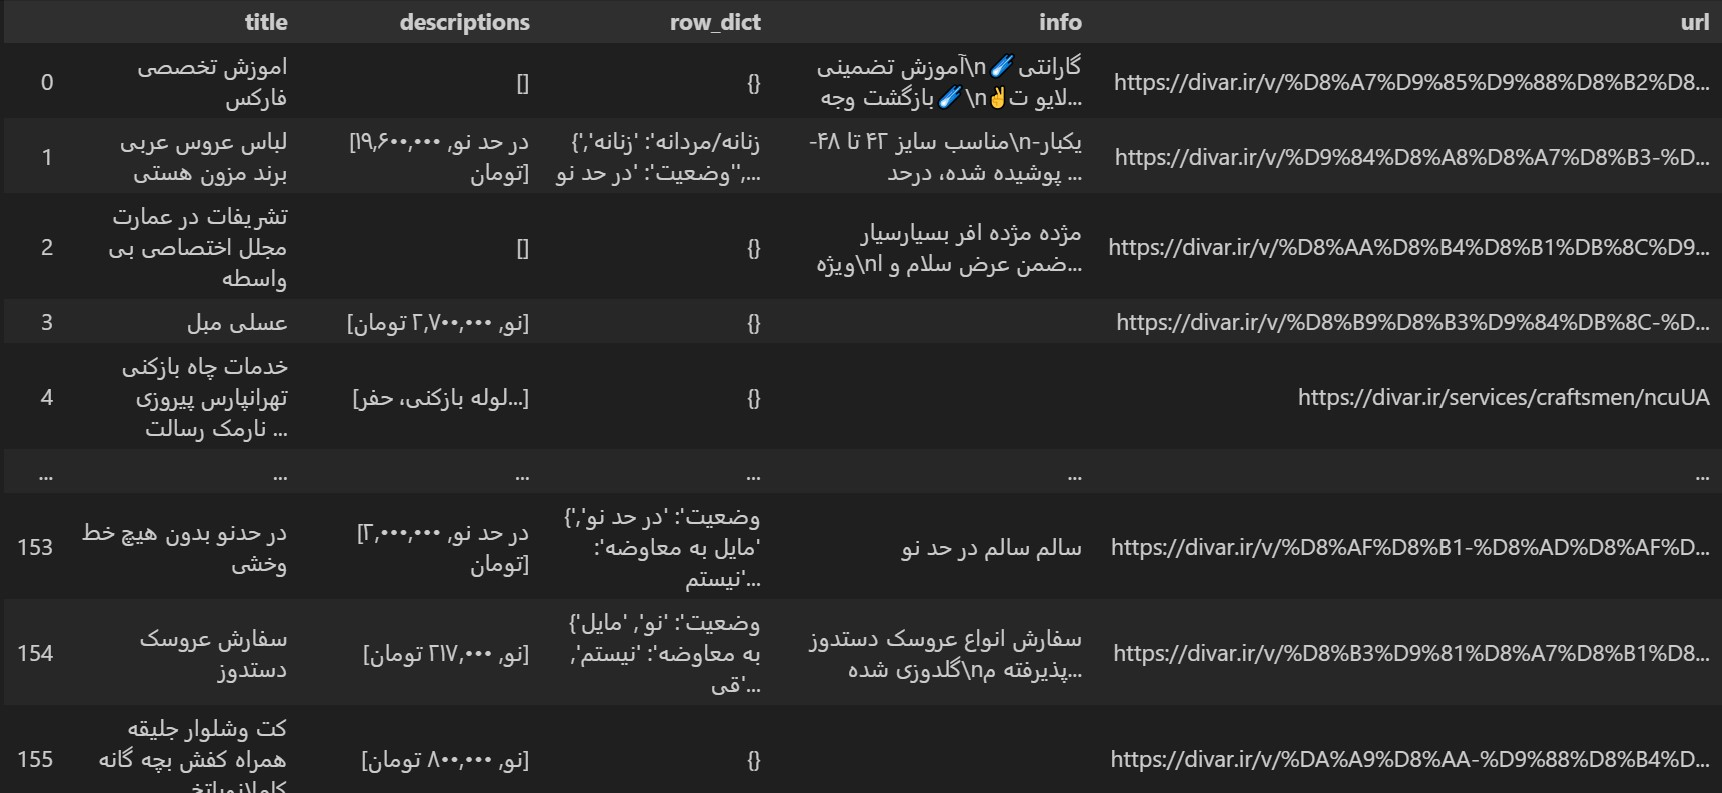
\includegraphics[width=1\textwidth]{Bonus.jpg}
    \caption{The extracted dataframe}
    \label{fig:bonus}
\end{figure}

\makeendpage
\end{document}